\documentclass{article}[a4paper]
\usepackage[utf8]{inputenc}
\usepackage[spanish]{babel}
\usepackage[a4paper, 11pt]{geometry}
\usepackage{graphicx}
\newcommand{\xor}{\oplus}
%\usepackage{xcolor}
\usepackage{listings} %code highlighter
\usepackage{blindtext}
\usepackage{titlesec}
\usepackage{appendix}
\usepackage[T1]{fontenc}
\usepackage{textcomp}
\usepackage{amssymb,amsmath}
\usepackage{hyperref}
\usepackage[dvipsnames]{xcolor}

\usepackage{listings}% http://ctan.org/pkg/listings
\lstset{
  basicstyle=\ttfamily,
  mathescape
}

\newcommand\tab[1][1cm]{\hspace*{#1}}

\definecolor{codegreen}{rgb}{0,0.6,0}
\definecolor{codegray}{rgb}{0.5,0.5,0.5}
\definecolor{codepurple}{rgb}{0.58,0,0.82}
\definecolor{backcolour}{rgb}{0.95,0.95,0.92}

\lstdefinestyle{mystyle}{
    backgroundcolor=\color{backcolour},   
    commentstyle=\color{codegreen},
    keywordstyle=\color{magenta},
    numberstyle=\tiny\color{codegray},
    stringstyle=\color{codepurple},
    basicstyle=\ttfamily\footnotesize,
    breakatwhitespace=false,         
    breaklines=true,                 
    captionpos=b,                    
    keepspaces=true,                 
    numbers=left,                    
    numbersep=5pt,                  
    showspaces=false,                
    showstringspaces=false,
    showtabs=false,                  
    tabsize=2
}

\lstset{style=mystyle}

\title{Memoria Práctica PDL: Analizador Sintáctico}
\author{Andrés Ollero Morales, Gabriel de Oliveira Trindade, Víctor Alejandro Sanz Ararat}
\date{Grupo 17}

\begin{document}

% \maketitle
\begin{titlepage}
   \begin{center}
       \vspace*{1cm}

       \textbf{Práctica Procesadores de Lenguajes}

       \vspace{0.5cm}
        Grupo 17
            
       \vspace{1.5cm}

        \textbf{Andrés Ollero Morales}\\
        \textbf{Víctor Alejandro Sanz Ararat}\\
        \textbf{Gabriel de Oliveira Trindade}\\

       \vfill
            
       \vspace{0.5cm}
     
       
\includegraphics[width=0.5\textwidth]{fiupm.png}

        \vfill
            
       \vspace{0.1cm}
       Departamento de Lenguajes y Sistemas Informáticos e Ingeniería de Software\\
       Escuela Técnica Superior De Ingenieros Informáticos\\
       Universidad Politécnica de Madrid\\
       Enero 2023
            
   \end{center}
\end{titlepage}
\thispagestyle{empty}
\newpage
\tableofcontents
\thispagestyle{empty}

\newpage

\section{Diseño final del Procesador}
La implementación fue realizada en el lenguaje de programación Java. Nuestro grupo contaba con las siguientes opciones de práctica:
\begin{itemize}
    \item Sentencias: Sentencia de selección múltiple (switch-case)
    \item Operadores especiales: Asignación con resto (\%=)
    \item Técnicas de Análisis Sintáctico: Descendente con tabla
    \item Comentarios: Comentario de bloque (/* */)
    \item Cadenas: Con comillas dobles (\" \")
\end{itemize}
De manera opcional, decidimos también implementar el token default para las sentencias switch-case.

\section{Diseño del Analizador Léxico}

\subsection{Diseño de Tokens}
\begin{verbatim}
        <palabraReservada, boolean>         <palabraReservada, input>
        <palabraReservada, break>           <palabraReservada, int>
        <palabraReservada, case>            <palabraReservada, let>
        <palabraReservada, function>        <palabraReservada, switch>
        <palabraReservada, print>           <palabraReservada, return>
        <palabraReservada, string>          <palabraReservada, if>
        <palabraReservada, default>
        
        <suma, >            <puntoComa, >       <asignacion, >
        <negacion, >        <coma, >            <dosPuntos, >
        <abrePar, >         <cierraPar, >       <comparacion, >
        <abreLlave, >       <cierraLlave, >     <asignacionResto, >
        <id, nºTS>          <constEnt, nº>      <cadena, "lexema">
\end{verbatim}

\subsection{Gramática Regular (Tipo III)}
\begin{verbatim}
    S -> "A | dB | %C | =D | _T | cT | {  |  }  |  (  |  )  |  +  |
          :  |  ;  |  ,  |  ! | del S
    T -> cT | _T | dT | O.C 
    A -> lA | " 
    B -> dB | O.C
    C -> =
    D -> = | O.C
    E -> \ E' | O.C
    E’ -> *E" | O.C E
    E’’ -> \ | O.C E'
    
    donde c = letras (a-z, A-Z), d = dígitos (0-9), l = cualquier cosa 
    y O.C = otro caracter distinto
\end{verbatim} 

\subsection{Autómata Finito Determinista}
\begin{figure}[h!]
\centering
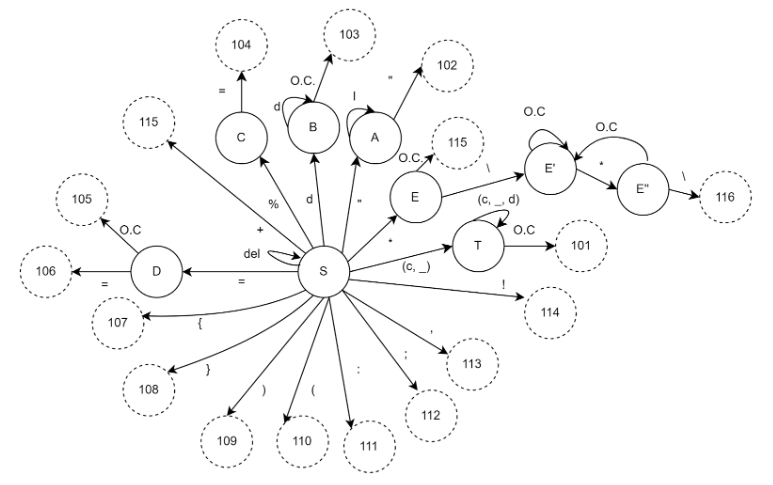
\includegraphics[width=0.9\textwidth]{automataAnLex.png}
\caption{\label{figura:automata}Implementación de la gramática con el autómata.}
\end{figure}

\subsection{Acciones Semánticas}
Se realiza la acción semántica LeerSigCaracter en todas las transiciones 
salvo en:
\begin{verbatim}
T : 101
B : 103
D : 105
S : T -> lexema = l; contador = 1;
T : T -> lexema = lexema + l; contador++;
T : 101 -> if (BuscarPalabraReservada(lexema) == 1) 
                then GenerarToken(palabraReservada, “”)
            else if (BuscarTablaSimbolos(lexema) == 1) 
                then GenerarToken(id, posTS)
            else (BuscarTablaSimbolos(lexema) == 0) 
                then AñadirEntradaTabla(id, posTS) && 
                    GenerarToken(palabraReservada, posTS);
S : A -> contador = 0; lexema = "";
A : A -> lexema = lexema + l; contador++;
A : 102 -> if (contador <= 64) 
                then GT(cadena, lexema)
	    else
	        then error(“longitud de la cadena excede el limite”);
S : B -> valor = valor_ascii(d);
B : B -> valor = valor + valor_ascii(d);
B : 103 -> if (valor <= 32767)
                then GenerarToken(constEnt, valor);
	    else
                then error(“valor del entero excede el limite”);
C : 104 -> if (c != ‘=’)
                then error(“expected '%=”);
           else
                GenerarToken(asignacionResto, );
D : 105 -> GenerarToken(igual, );
D : 106 -> GenerarToken(comparación, );
S : 107 -> GenerarToken(abreLlave, );
S : 108 -> GenerarToken(cierraLlave, );
S : 109 -> GenerarToken(abrePar, );
S : 110 -> GenerarToken(cierraPar, );
S : 111 -> GenerarToken(dosPuntos, );
S : 112 -> GenerarToken(puntoComa, );
S : 113 -> GenerarToken(coma, );
S : 114 -> GenerarToken(negación, );
S : 115 -> GenerarToken(suma, );

- GenerarToken (atributo, valor): Genera el token en un fichero de 
                                  salida tokens.txt.
- BuscarPalabraReservada (lexema): Busca la palabra reservada en la 
                                   respectiva tabla de palabras reservada.
- AñadirEntradaTabla(lexema, posTS): Añadimos el nombre de la variable a 
                                     la tabla de símbolos.
\end{verbatim}

\subsection{Errores}
Cuando se introduce en el código un símbolo que no pertenece al lenguaje, nuestro autómata lo omite. Los errores que contempla el código son cuando (y su correspondiente mensaje por línea de comandos):\\

- Se crea un identificador que no empieza por letra o subrayado.\\
\tab \tab \textcolor{red}{Error en línea: n -> Error Léxico: inicio de nombre de variable inválido.}

- Se introduce un número entero superior a 32767.\\
\tab \tab \textcolor{red}{Error en línea: n -> Error Léxico: el valor numerico excede el límite de 32767.}

- Se intenta crear una cadena de más de 64 caracteres.\\
\tab \tab \textcolor{red}{Error en línea: n -> Error Léxico: Cadena sobrepasa los 64 caracteres.}

- Se crea una cadena sin finalizar con la doble comilla final.\\
\tab \tab \textcolor{red}{Error: La string esta mal formada.}

- Se introduce exclusivamente un '\%' sin el caracter '=' a continuación.\\
\tab \tab \textcolor{red}{Error: Expected '=' after '\%'.}

- Se intenta hacer comentario de bloque y no se introducen los /* */ correctamente.\\
\tab \tab \textcolor{red}{Error en línea: n -> Error Léxico: Fin de comentario no válido.}\\

Y por supuesto, no se genera el token.


\newpage

\section{Diseño del Analizador Sintáctico}
\subsection{Gramática de Contexto Libre (Tipo II)}
Para ello hemos tomado la gramática que venía dada en las diapositivas de la explicación de la práctica modificándola a los terminales que escogimos al inicio. Eliminamos la recursividad por la izquierda y la factorizamos para cumplir la condición LL(1).

\begin{verbatim}
Axioma = PP

NoTerminales = { PP P S SS E R RR U UU V VV L Q X B T A K C F H O D }

Terminales = { ! == + id ( ) constEnt cadena %= print input return , if break 
                switch case int boolean string let function ; : = { } default }

Producciones = {
    E -> R RR
    RR -> == R RR
    RR -> lambda
    R -> U UU
    UU -> + U UU
    UU -> lambda
    U -> ! V
    U -> V
    V -> id VV
    V -> ( E )
    V -> constEnt
    V -> cadena
    VV -> ( L )
    VV -> lambda
    S -> id SS
    SS -> %= E ;
    SS -> = E ;
    SS -> ( L ) ;
    S -> print R ;
    S -> input id ;
    S -> return X ;
    L -> E Q
    L -> lambda
    Q -> , E Q
    Q -> lambda
    X -> E
    X -> lambda
    B -> switch ( E ) { O }
    B -> if ( E ) S
    O -> case constEnt : C D O
    O -> default : C D O
    O -> lambda
    D -> break ;
    D -> lambda
    B -> let id T ;
    T -> int
    T -> boolean
    T -> string
    B -> S
    F -> function id H ( A ) { C }
    H -> T
    H -> lambda
    A -> T id K
    A -> lambda
    K -> , T id K
    K -> lambda
    C -> B C
    C -> lambda
    P -> B P
    P -> F P
    P -> lambda
    PP -> P
}
\end{verbatim}

\subsection{First y Follow}
\begin{verbatim}
First(E) = {!, id, (, constEnt, cadena}
First(R) = {!, id, (, constEnt, cadena}
First(RR) = {==, lambda} 
First(U) = {!, id, (, constEnt, cadena}
First(UU) = {+, lambda}
First(V) = {id, (, constEnt, cadena}
First(VV) = {(, lambda}
First(S) = {id, print, input, return}
First(SS) = {%, =, (}
First(L) = {!, id, (, constEnt, cadena, lambda}
First(Q) = {‘,’ , lambda}
First(X) = {!, id, (, constEnt, cadena, lambda}
First(B) = {switch, let, if, id, print, input, return}
First(O) = {case, default, lambda}
First(D) = {break, lambda}
First(T) = {int, boolean, string}
First(F) = {function}
First(H) = {function, lambda}
First(A) = {function, lambda}
First(K) = {‘,’ , lambda}
First(C) = {switch, let, if, id, print, input, return, lambda}
First(P) = {function, switch, let, if, id, print, input, return, lambda}
First(PP) = First(P)

Follow(E) = {), ;, ‘,’}
Follow(R) = {==}
Follow(RR) = {), ;, ‘,’}
Follow(U) = {+}
Follow(UU) = {==}
Follow(V) = {+} 
Follow(VV) = {+}
Follow(S) = {function, switch, let, if, id, print, input, return}
Follow(SS) = {function, switch, let, if, id, print, input, return}
Follow(L) = { ) }
Follow(Q) = { ) }
Follow(X) = { ; }
Follow(B) = {function, switch, let, if, id, print, input, return}
Follow(O) = { } }
Follow(D) = {case, default}
Follow(T) = {;, id, (}
Follow(F) = {function, switch, let, if, id, print, input, return}
Follow(H) = { ( }
Follow(A) = { ) } 
Follow(K) = { ) }
Follow(C) = { } }
Follow(P) = {$}
Follow(PP) = {$}
\end{verbatim}

\subsection{Demostración LL1}
Para las 52 reglas de producción, hallamos que para cada No Terminal que tenga más de una producción en la gramática:\\
1. No exista ningún terminal se deriven de los No Terminales y sea la primera aparición (la intersección de sus firsts sea vacía).\\
2. Si un No Terminal se puede derivar a Lambda, el terminal producido por la regla no puede estar contenido en su follow.\\

Los no terminales que contienen dos o más producciones son: RR, UU, U, V, VV, S, SS, L, Q, X, B, O, D, T, H, A, K, C, P.\\ \\

\textbf{RR:}\\
\tab RR $\rightarrow$ == R RR\\ 
\tab RR $\rightarrow$ $\lambda$\\ \\
\tab \tab First(= R RR) $\cap$ First($\lambda$) = $\lbrace$==$\rbrace$ $\cap$ $\lbrace$$\lambda$$\rbrace$ $\rightarrow$ al aparecer $\lambda$:\\
\tab \tab First(== R RR) $\cap$ Follow(RR) = $\lbrace$==$\rbrace$ $\cap$ $\lbrace$), ;, ','$\rbrace$ = $\emptyset$\\

\textbf{UU:}\\
\tab UU $\rightarrow$ + U UU\\ 
\tab UU $\rightarrow$ $\lambda$\\ \\
\tab \tab First(+ U UU) $\cap$ First($\lambda$) = $\lbrace$+$\rbrace$ $\cap$ $\lbrace$$\lambda$$\rbrace$ $\rightarrow$ al aparecer $\lambda$:\\
\tab \tab First(+ U UU) $\cap$ Follow(UU) = $\lbrace$+$\rbrace$ $\cap$ $\lbrace$==$\rbrace$ = $\emptyset$\\ \\

\textbf{U:}\\
\tab U $\rightarrow$ ! V\\
\tab U $\rightarrow$ V\\ \\
\tab \tab First(!V) $\cap$ First(V) = $\lbrace$!$\rbrace$ $\cap$ $\lbrace$id, (, constEnt, cad$\rbrace$ = $\emptyset$\\

\textbf{V:}\\
\tab V $\rightarrow$ id VV\\
\tab V $\rightarrow$ ( E )\\
\tab V $\rightarrow$ constEnt\\
\tab V $\rightarrow$ cadena\\ \\
\tab \tab First(id VV) $\cap$ First( ( E ) ) = $\lbrace$id$\rbrace$ $\cap$ $\lbrace$($\rbrace$ = $\emptyset$\\
\tab \tab First(id VV) $\cap$ First(constEnt) = $\lbrace$id$\rbrace$ $\cap$ $\lbrace$constEnt$\rbrace$ = $\emptyset$\\
\tab \tab First(id VV) $\cap$ First(cadena) = $\lbrace$id$\rbrace$ $\cap$ $\lbrace$cadena$\rbrace$ = $\emptyset$\\
\tab \tab First( ( E ) ) $\cap$ First(constEnt) = $\lbrace$($\rbrace$ $\cap$ $\lbrace$constEnt$\rbrace$ = $\emptyset$\\
\tab \tab First( ( E ) ) $\cap$ First(cadena) = $\lbrace$($\rbrace$ $\cap$ $\lbrace$cadena$\rbrace$ = $\emptyset$\\
\tab \tab First(constEnt) $\cap$ First(cadena) = $\lbrace$constEnt$\rbrace$ $\cap$ $\lbrace$cadena$\rbrace$ = $\emptyset$\\

\textbf{VV:}\\
\tab VV $\rightarrow$ ( L )\\
\tab VV $\rightarrow$ $\lambda$\\ \\
\tab \tab First( ( L ) ) $\cap$ First($\lambda$) = $\lbrace$($\rbrace$ $\cap$ $\lbrace$$\lambda$$\rbrace$ $\rightarrow$ al aparecer $\lambda$:\\
\tab \tab First( ( L ) ) $\cap$  Follow(VV) = $\lbrace$($\rbrace$ $\cap$ $\lbrace$+$\rbrace$ = \emptyset \\

\textbf{S:}\\
\tab S $\rightarrow$ id SS\\
\tab S $\rightarrow$ print R ;\\
\tab S $\rightarrow$ input id ;\\
\tab S $\rightarrow$ return X ;\\ \\
\tab \tab First(id SS) $\cap$ First(print R ;) = $\lbrace$id$\rbrace$ $\cap$ $\lbrace$print$\rbrace$ = $\emptyset$\\
\tab \tab First(id SS) $\cap$ First(input id ;) = $\lbrace$id$\rbrace$ $\cap$ $\lbrace$input$\rbrace$ = $\emptyset$\\
\tab \tab First(id SS) $\cap$ First(return X) = $\lbrace$id$\rbrace$ $\cap$ $\lbrace$return$\rbrace$ = $\emptyset$\\
\tab \tab First(print R ;) $\cap$ First(input id ;) = $\lbrace$print$\rbrace$ $\cap$ $\lbrace$input$\rbrace$ = $\emptyset$\\
\tab \tab First(print R ;) $\cap$ First(return X ;) = $\lbrace$print$\rbrace$ $\cap$ $\lbrace$return$\rbrace$ = $\emptyset$\\
\tab \tab First(input id ;) $\cap$ First(return X ;) = $\lbrace$input$\rbrace$ $\cap$ $\lbrace$return$\rbrace$ = $\emptyset$\\

\textbf{SS:}\\
\tab SS $\rightarrow$ \%= E ;\\
\tab SS $\rightarrow$ = E ;\\
\tab SS $\rightarrow$ ( L )\\ \\
\tab \tab First(\%= E) $\cap$ First(= E ;) = $\lbrace$\%=$\rbrace$ $\cap$ $\lbrace$=$\rbrace$ = $\emptyset$\\
\tab \tab First(\%= E) $\cap$ First( ( L ) ) = $\lbrace$\%=$\rbrace$ $\cap$ $\lbrace$($\rbrace$ = $\emptyset$\\
\tab \tab First(= E ;) $\cap$ First( ( L ) ) = $\lbrace$=$\rbrace$ $\cap$ $\lbrace$($\rbrace$ = $\emptyset$\\ \\

\textbf{L:}\\
\tab L $\rightarrow$ E Q\\
\tab L $\rightarrow$ $\lambda$\\ \\
\tab \tab First(E Q) $\cap$ First($\lambda$) = $\lbrace$!, id, (, constEnt, cadena$\rbrace$ $\cap$ $\lbrace$$\lambda$$\rbrace$$\rightarrow$ al aparecer $\lambda$:\\
\tab \tab First(E Q) $\cap$ Follow(L) = $\lbrace$!, id, (, constEnt, cadena$\rbrace$ $\cap$ $\lbrace$)$\rbrace$ = $\emptyset$\\

\textbf{Q:}\\
\tab Q $\rightarrow$ , E Q\\
\tab Q $\rightarrow$ $\lambda$\\ \\
\tab \tab First(, E Q) $\cap$ First($\lambda$) = $\lbrace$,$\rbrace$ $\cap$ $\lbrace$$\lambda$$\rbrace$$\rightarrow$ al aparecer $\lambda$:\\
\tab \tab First(, E Q) $\cap$ Follow(Q) = $\lbrace$,$\rbrace$ $\cap$ $\lbrace$)$\rbrace$ = $\emptyset$\\

\textbf{X:}\\
\tab X $\rightarrow$ E\\
\tab E $\rightarrow$ $\lambda$\\ \\
\tab \tab First(E) $\cap$ First($\lambda$) = $\lbrace$!, id, (, constEnt, cadena$\rbrace$ $\cap$ $\lbrace$$\lambda$$\rbrace$ $\rightarrow$ al aparecer $\lambda$:\\
\tab \tab First(E) $\cap$ Follow(X) = $\lbrace$!, id, (, constEnt, cadena$\rbrace$ $\cap$ $\lbrace$;$\rbrace$ = \emptyset \\

\textbf{B:}\\
\tab B $\rightarrow$ switch ( E ) $\lbrace$ O $\rbrace$\\
\tab B $\rightarrow$ if ( E ) S \\
\tab B $\rightarrow$ let id T ;\\
\tab B $\rightarrow$ S\\ \\
\tab \tab First(switch ( E ) $\lbrace$ O $\rbrace$) $\cap$ First(if ( E ) S) = $\lbrace$switch$\rbrace$ $\cap$ $\lbrace$if$\rbrace$ = $\emptyset$\\
\tab \tab First(switch ( E ) $\lbrace$ O $\rbrace$) $\cap$ First(let id T ;) = $\lbrace$switch$\rbrace$ $\cap$ $\lbrace$let$\rbrace$ = $\emptyset$\\
\tab \tab First(switch ( E ) $\lbrace$ O $\rbrace$) $\cap$ First(S) = $\lbrace$switch$\rbrace$ $\cap$ $\lbrace$id, print, input, return$\rbrace$ = $\emptyset$\\
\tab \tab First(if ( E ) S) $\cap$ First(let id T ;) = $\lbrace$if$\rbrace$ $\cap$ $\lbrace$let$\rbrace$ = $\emptyset$\\
\tab \tab First(if ( E ) S) $\cap$ First(S) = $\lbrace$if$\rbrace$ $\cap$ $\lbrace$id, print, input, return$\rbrace$ = $\emptyset$\\
\tab \tab First(let id T ;) $\cap$ First(S) = $\lbrace$let$\rbrace$ $\cap$ $\lbrace$id, print, input, return$\rbrace$ = $\emptyset$\\

\textbf{O:}\\
\tab O $\rightarrow$ case constEnt : C D O\\
\tab O $\rightarrow$ default: C D O\\
\tab O $\rightarrow$ $\lambda$\\ \\
\tab \tab First(case constEnt: CDO) $\cap$ First(default: CDO) = $\lbrace$case$\rbrace$ $\cap$ $\lbrace$default$\rbrace$ = $\emptyset$\\
\tab \tab First(case constEnt : C D O) $\cap$ First($\lambda$) = $\lbrace$case$\rbrace$ $\cap$ $\lbrace$$\lambda$$\rbrace$ $\rightarrow$ al aparecer $\lambda$:\\
\tab \tab First(case constEnt : C D O) $\cap$ Follow(O) = $\lbrace$case$\rbrace$ $\cap$ $\lbrace$$\rbrace$$\rbrace$ = $\emptyset$\\
\tab \tab First(default : C D O) $\cap$ First($\lambda$) = $\lbrace$case$\rbrace$ $\cap$ $\lbrace$$\lambda$$\rbrace$ $\rightarrow$ al aparecer $\lambda$:\\
\tab \tab First(default : C D O) $\cap$ Follow(O) = $\lbrace$case$\rbrace$ $\cap$ $\lbrace$$\rbrace$$\rbrace$ = $\emptyset$\\

\textbf{D:}\\
\tab D $\rightarrow$ break ;\\
\tab D $\rightarrow$ $\lambda$\\ \\
\tab \tab First(break ;) $\cap$ First($\lambda$) = $\lbrace$break$\rbrace$ $\cap$ $\lbrace$$\lambda$$\rbrace$ $\rightarrow$ al aparecer $\lambda$:\\
\tab \tab First(break ;) $\cap$ Follow(D) = $\lbrace$break$\rbrace$ $\cap$ $\lbrace$case, default$\rbrace$ = $\emptyset$\\

\textbf{T:}\\
\tab T $\rightarrow$ int\\
\tab T $\rightarrow$ boolean\\
\tab T $\rightarrow$ string\\ \\
\tab \tab First(int) $\cap$ First(boolean) = $\lbrace$int$\rbrace$ $\cap$ $\lbrace$boolean$\rbrace$ = $\emptyset$\\
\tab \tab First(int) $\cap$ First(string) = $\lbrace$int$\rbrace$ $\cap$ $\lbrace$string$\rbrace$ = $\emptyset$\\
\tab \tab First(boolean) $\cap$ First(string) = $\lbrace$boolean$\rbrace$ $\cap$ $\lbrace$string$\rbrace$ = $\emptyset$\\

\textbf{H:}\\
\tab H $\rightarrow$ T\\
\tab H $\rightarrow$ $\lambda$\\ \\
\tab \tab First(T) $\cap$ First($\lambda$) = $\lbrace$int, boolean, string$\rbrace$ $\cap$ $\lbrace$$\lambda$$\rbrace$ $\rightarrow$ al aparecer $\lambda$:\\
\tab \tab First(T) $\cap$ Follow(H) = $\lbrace$int, boolean, string$\rbrace$ $\cap$ $\lbrace$($\rbrace$ = $\emptyset$\\

\textbf{A:}\\
\tab A $\rightarrow$ T id K\\
\tab A $\rightarrow$ $\lambda$\\ \\
\tab \tab First(T id K) $\cap$ First($\lambda$) = $\lbrace$int, boolean, string$\rbrace$ $\cap$ $\lbrace$$\lambda$$\rbrace$ $\rightarrow$ al aparecer $\lambda$:\\
\tab \tab First(T id K) $\cap$ Follow(A) = $\lbrace$int, boolean, string $\rbrace$ $\cap$ $\lbrace$)$\rbrace$ = $\emptyset$\\

\textbf{K:}\\
\tab K $\rightarrow$ , T id K\\
\tab K $\rightarrow$ $\lambda$\\ \\
\tab \tab First(, T id K) $\cap$ First($\lambda$) = $\lbrace$,$\rbrace$ $\cap$ $\lbrace$$\lambda$$\rbrace$ $\rightarrow$ al aparecer $\lambda$:\\
\tab \tab First(, T id K) \cap  Follow(K) = $\lbrace$,$\rbrace$ $\cap$ $\lbrace$)$\rbrace$ = $\emptyset$\\

\textbf{C:}\\
\tab C $\rightarrow$ B C\\
\tab C $\rightarrow$ $\lambda$\\ \\
\tab \tab First(B C) $\cap$ First($\lambda$) = $\lbrace$switch, let, if, id, print, input, return$\rbrace$ $\cap$ $\lbrace$$\lambda$$\rbrace$ $\rightarrow$\\
\tab \tab First(B C) $\cap$  Follow(C) = $\lbrace$switch, let, if, id, print, input, return$\rbrace$ $\cap$ $\lbrace$$\rbrace$$\rbrace$ = $\emptyset$\\

\textbf{P:}\\
\tab P $\rightarrow$ B P\\
\tab P $\rightarrow$ F P\\
\tab P $\rightarrow$ $\lambda$\\ \\
\tab \tab First(BP)$\cap$First(FP)=$\lbrace$switch, let, if, id, print, input, return$\rbrace$$\cap$$\lbrace$function$\rbrace$ = $\emptyset$\\
\tab \tab First(B P) $\cap$ First(F P) = $\lbrace$switch, let, if, id, print, input, return$\rbrace$ $\cap$ $\lbrace$$\lambda$$\rbrace$ $\rightarrow$\\
\tab \tab First(B P) $\cap$ Follow(P) = $\lbrace$switch, let, if, id, print, input, return$\rbrace$ $\cap$ $\lbrace$\$$\rbrace$ = $\emptyset$\\
\tab \tab First(F P) $\cap$ First($\lambda$) = $\lbrace$function$\rbrace$ $\cap$ $\lbrace$$\lambda$$\rbrace$ $\rightarrow$\\
\tab \tab First(F P) $\cap$ Follow(P) = $\lbrace$function$\rbrace$ $\cap$ $\lbrace$\$$\rbrace$ = $\emptyset$\\

\subsection{Tabla de Análisis}
Utilizamos la herramienta Sistema Generador de Gramáticas LL1, donde introdujimos la gramática factorizada, sin recursividad por la izquierda, y nos produjo la siguiente tabla, que le indica al Analizador Sintáctico que reglas aplicar según los tokens que reciba.
\begin{figure}[h!]
\centering
\href{https://docs.google.com/spreadsheets/d/17yF_afvRGqVFFo7q70U3LPK74hVvpB8d/edit#gid=2045406742}{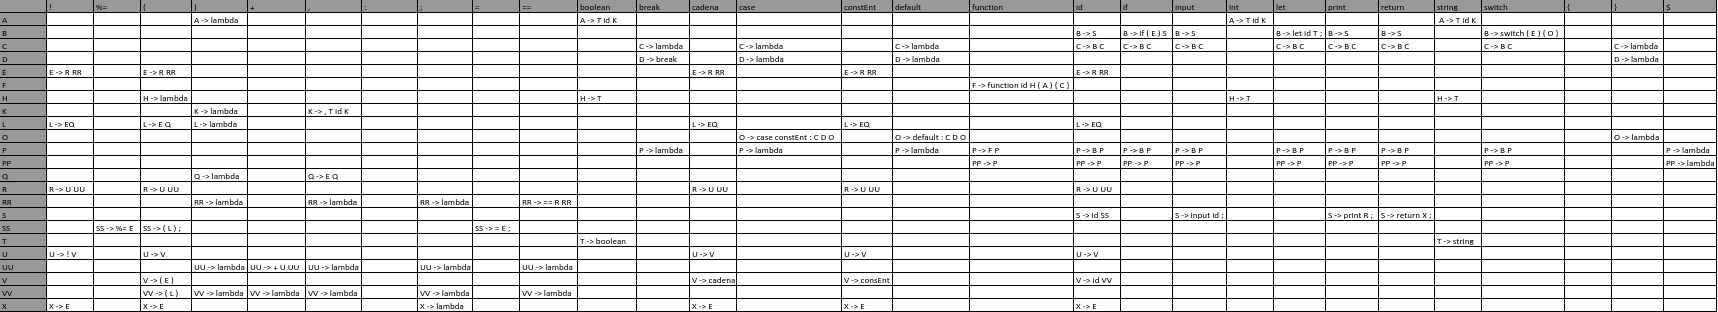
\includegraphics[width=1\textwidth]{tablaM.png}}
\caption{\label{figura:tablaM}Tabla de Análisis de LL1 (Click para una hoja de cálculo con mayor resolución).}
\end{figure}

\newpage

\section{Diseño del Analizador Semántico}

\subsection{Traducción Dirigida Por la Sintáxis}
Implementamos un Esquema de Traducción (EdT) sobre la Gramática de Contexto Libre del Analizador Sintáctico:\\

\noindent\textbf{Variables:}\\
\tab TSG = Tabla de Símbolos Global\\
\tab DespG = Desplazamiento de la TS Global\\
\tab TSActual = Tabla de Símbolos Actual\\
\tab TSL = Tabla de Símbolos Local\\
\tab DespL = Desplazamiento de la TS Local\\
\tab ZonaDecl = Zona Declarativa\\

\noindent\textbf{Métodos:}\\
\tab crearTS()\\
\tab destruirTS(TSi)\\
\tab insertaTipoTS(posicion de X, tipo de X)\\
\tab insertaEtTS(posicion de X, nueva etiqueta para la TS)\\
\tab nuevaEt() \textcolor{gray}{//las funciones no tienen desplazamiento en la TSG, sino una etiqueta}\\
\tab tipoDeFunción() \textcolor{gray}{//devuelve el tipo de la función actual}\\
\tab buscaTipoTS(posicion de X)\\
\tab initCases() \textcolor{gray}{//comprueba que cada case del switch no repita el numero}\\

\noindent\underline{Bloque Axioma:}\\

\tab PP $\rightarrow$ \textcolor{OliveGreen}{$ $\lbrace$TSG:= crearTS(), DespG := 0, TSActual := TSG$\rbrace$_{1.1}$} P \textcolor{OliveGreen}{$ $\lbrace$destruirTS(TSG)$\rbrace$_{1.2}$}\\

\tab P $\rightarrow$ B P \textcolor{OliveGreen}{$ $\lbrace$if (P2.tipo = tipo.vacio \&\& B.tipo = tipo.ok)\\ \tab \tab \tab \tab
then P.tipo := tipo.ok\\ \tab \tab \tab
else if (P2.tipo = tipo.ok \&\& B.tipo = tipo.ok)\\ \tab \tab \tab \tab
then P.tipo:= tipo.ok\\ \tab \tab \tab
else then\\ \tab \tab \tab \tab
P.tipo := tipo.error;\\ \tab \tab \tab
POP(2)$\rbrace$_{2}$}\\

\tab P $\rightarrow$ \textcolor{OliveGreen}{$ $\lbrace$ZonaDecl := true$\rbrace$_{3.1}$}
F P \textcolor{OliveGreen}{$ $\lbrace$if (P2.tipo = tipo.vacio \&\& F.tipo = tipo.ok) \\ \tab \tab \tab \tab
then P.tipo := tipo.ok \\ \tab \tab \tab
else if (P2.tipo = tipo.ok \&\& F.tipo = tipo.ok) \\ \tab \tab \tab \tab
then P.tipo:= tipo.ok \\ \tab \tab \tab
else then\\ \tab \tab \tab \tab
P.tipo := tipo.error;\\ \tab \tab \tab
POP(2)$\rbrace$_{3.2}$}\\

\tab P $\rightarrow$ $\lambda$ \textcolor{OliveGreen}{$ $\lbrace$P.tipo := tipo.vacío$\rbrace$_{4}$}\\ \\ \\ %saltos de linea!!!!!!!!!!!!!!!!!!!!!!!!!!!



\noindent\underline{Bloque declaración de funciones:}\\

\tab F $\rightarrow$ function id \textcolor{OliveGreen}{$ $\lbrace$TSL := crearTS(), DespL := 0$\rbrace$ _{5.1}$} \\ \tab \tab
H ( A ) \textcolor{OliveGreen}{$ $\lbrace$insertaTipoTS(id.pos, H.tipo); insertaEtTS(id.pos, nuevaEt())$\rbrace$_{5.2}$} \\ \tab \tab
$\lbrace$ C \textcolor{OliveGreen}{$ $\lbrace$destruirTS(TSL)$\rbrace$_{5.3}$}$\rbrace$ \\ \tab \tab \tab \textcolor{OliveGreen}{$ $\lbrace$if (C.tipo != tipo.ok \&\& C.tipo != tipo.vacío) \\ \tab \tab \tab \tab
then error(“tipos de return y función no coincide”)\\ \tab \tab \tab
else F.tipo := tipo.ok\\ \tab \tab \tab
POP(9)$\rbrace$_{5.4}$}\\

\tab H $\rightarrow$ T \textcolor{OliveGreen}{$ $\lbrace$H.tipo := T.tipo; POP(1)$\rbrace$_{6}$}\\

\tab H $\rightarrow$ $\lambda$ \textcolor{OliveGreen}{$ $\lbrace$H.tipo := tipo.vacío$\rbrace$_{7}$}\\

\tab A $\rightarrow$ T id K \textcolor{OliveGreen}{$ $\lbrace$A.tipo := T.tipo, insertaTipoTS(id.pos, T.tipo), insertaDespTS(id.pos, DespL), DespL := DespL + T.ancho; POP(3)$\rbrace$_{8}$}\\

\tab A $\rightarrow$ $\lambda$ \textcolor{OliveGreen}{$ $\lbrace$A.tipo := tipo.vacío$\rbrace$_{9}$}\\

\tab K $\rightarrow$ , T id K \textcolor{OliveGreen}{$ $\lbrace$K.tipo := T.tipo, insertaTipoTS(id.pos, T.tipo), insertaDespTS(id.pos, DespL), DespL := DespL + T.ancho; POP(4)$\rbrace$_{10}$}\\

\tab K $\rightarrow$ $\lambda$ \textcolor{OliveGreen}{$ $\lbrace$K.tipo := tipo.vacio$\rbrace$_{11}$}\\

\tab C $\rightarrow$ B C \textcolor{OliveGreen}{$ $\lbrace$if(C2.tipo = tipo.vacio) \\ \tab \tab \tab \tab
then C.tipo = B.tipo \\ \tab \tab \tab
else C.tipo = C2.tipo\\ \tab \tab \tab
POP(2)$\rbrace$_{12}$}\\

\tab C $\rightarrow$ $\lambda$ \textcolor{OliveGreen}{$ $\lbrace$C.tipo := tipo.vacío$\rbrace$_{13}$}\\


\noindent\underline{Bloque sentencias compuestas y declaración de variables:}\\

\tab B $\rightarrow$ if ( E ) S \textcolor{OliveGreen}{$ $\lbrace$if (E.tipo == boolean \&\& S.tipo != tipo.vacio) \\ \tab \tab \tab \tab \tab
then B.tipo := tipo.ok  \\ \tab \tab \tab \tab
else B.tipo := tipo.error\\ \tab \tab \tab \tab
POP(5)$\rbrace$_{14}$}\\

\tab B $\rightarrow$ switch \textcolor{OliveGreen}{$ $\lbrace$initCases()$\rbrace$_{15.1}$}\\ \tab \tab \tab
( E ) \textcolor{OliveGreen}{$ $\lbrace$if (E.tipo = tipo.ok) \\ \tab \tab \tab \tab \tab
then B := tipo.ok \\ \tab \tab \tab \tab
else B.tipo := tipo.error)$\rbrace$_{15.2}$}\\ \tab \tab \tab
$\lbrace$ O $\rbrace$ \textcolor{OliveGreen}{$ $\lbrace$if (E.tipo := constEnt \&\& tipo.O := tipo.ok) \\ \tab \tab \tab \tab \tab
then B.tipo := tipo.ok \\ \tab \tab \tab \tab
else B.tipo := tipo.error\\ \tab \tab \tab \tab
POP(7)$\rbrace$_{15.3}$}\\ \\ \\

\tab O $\rightarrow$ case constEnt \textcolor{OliveGreen}{$ $\lbrace$if(comprobarCases(constEnt) = true)\\ \tab \tab \tab \tab \tab
then añadirCases(constEnt)\\ \tab \tab \tab \tab 
else error("uno o multiples casos con el mismo valor")$\rbrace$_{16.1}$} \\ \tab \tab
 : C D O \textcolor{OliveGreen}{$ $\lbrace$if (C.tipo = tipo.ok || C.tipo = tipo.vacio) \&\& (O2.tipo = tipo.ok ||  \\ \tab \tab \tab \tab
 O2.tipo = tipo.vacio)) \\ \tab \tab \tab \tab \tab
then O.tipo := tipo.ok \\ \tab \tab \tab \tab
else then O.tipo := tipo.error\\ \tab \tab \tab \tab
POP(6)$\rbrace$_{16.2}$}\\

\tab O $\rightarrow$ default : C D O \textcolor{OliveGreen}{$ $\lbrace$if (C.tipo = tipo.ok \&\& (O2.tipo = tipo.ok || \\ \tab \tab \tab \tab \tab O2.tipo = tipo.vacio)) \\ \tab \tab \tab \tab \tab \tab
then O.tipo := tipo.ok\\ \tab \tab \tab \tab \tab
else then O.tipo := tipo.error\\ \tab \tab \tab \tab
POP(5)$\rbrace$_{17}$}\\
   
\tab O $\rightarrow$ $\lambda$ \textcolor{OliveGreen}{$ $\lbrace$O.tipo := tipo.vacío$\rbrace$_{18}$}\\

\tab D $\rightarrow$ break ; \textcolor{OliveGreen}{$ $\lbrace$D.tipo := tipo.ok; POP(2)$\rbrace$_{19}$}\\

\tab D $\rightarrow$ $\lambda$ \textcolor{OliveGreen}{$ $\lbrace$D.tipo := tipo.vacio$\rbrace$_{20}$}\\

\tab B $\rightarrow$ \textcolor{OliveGreen}{$ $\lbrace$ZonaDecl = true$\rbrace$_{21.1}$}
let id T \textcolor{OliveGreen}{$ $\lbrace$ZonaDecl = false$\rbrace$_{21.2}$}\\ \tab \tab
; \textcolor{OliveGreen}{$ $\lbrace$B.tipo := tipo.ok \\ \tab \tab \tab
if (TSL = null) \\ \tab \tab \tab \tab
insertaTipoTSL(id.pos, T.tipo), insertaDespTSL(id.pos, DespL),\\ \tab \tab \tab \tab
DespL := DespL + T.ancho
\\ \tab \tab \tab
else \\ \tab \tab \tab \tab
insertaTipoTSG(id.pos, T.tipo), insertaDespTSG(id.pos, DespL),\\ \tab \tab \tab \tab
DespG := DespG + T.ancho\\ \tab \tab \tab
POP(4)$\rbrace$_{21.3}$}\\

\tab T $\rightarrow$ int \textcolor{OliveGreen}{$ $\lbrace$T.tipo = constEnt; POP(1)$\rbrace$_{22}$}\\

\tab T $\rightarrow$ boolean \textcolor{OliveGreen}{$ $\lbrace$T.tipo = boolean; POP(1)$\rbrace$_{23}$}\\

\tab T $\rightarrow$ string \textcolor{OliveGreen}{$ $\lbrace$T.tipo = cadena; POP(1)$\rbrace$_{24}$}\\

\tab B $\rightarrow$ S \textcolor{OliveGreen}{$ $\lbrace$if (S.tipo != tipo.error \&\& S.tipo != tipo.vacio)) \\ \tab \tab \tab \tab
then B.tipo := tipo.ok \\ \tab \tab \tab
else B.tipo := tipo.error\\ \tab \tab \tab POP(1)$\rbrace$_{25}$}\\


\noindent\underline{Sentencias simples:}\\

\tab S $\rightarrow$ id SS \textcolor{OliveGreen}{$ $\lbrace$if (SS.tipo = tipo.ok || (buscaTipoTSL(id.pos) != null \&\& \\ \tab \tab \tab SS.tipo = buscaTipoTSL(id.pos))) \\ \tab \tab \tab \tab \tab
then S.tipo:=tipo.ok \\ \tab \tab \tab \tab 
else if (SS.tipo = tipo.ok || (buscaTipoTSG(id.pos) != null \&\& \\ \tab \tab \tab \tab \tab SS.tipo = buscaTipoTSG(id.pos))) \\ \tab \tab \tab \tab \tab
then S.tipo:=tipo.ok \\ \tab \tab \tab \tab 
else S.tipo := tipo.error\\ \tab \tab \tab \tab
POP(2)$\rbrace$_{26}$}\\

 \tab SS $\rightarrow$ \%= E ; \textcolor{OliveGreen}{$ $\lbrace$if (E.tipo = constEnt) \\ \tab \tab \tab \tab \tab
then SS.tipo := tipo.ok \\ \tab \tab \tab \tab
else SS.tipo := tipo.error\\ \tab \tab \tab \tab
POP(3)$\rbrace$_{27}$}\\

\tab SS $\rightarrow$ = E ; \textcolor{OliveGreen}{$ $\lbrace$if (E.tipo != tipo.error \&\& E.tipo != tipo.vacio) \\ \tab \tab \tab \tab \tab
then SS.tipo := E.tipo \\ \tab \tab \tab \tab
else SS.tipo := tipo.error\\ \tab \tab \tab \tab
POP(3)$\rbrace$_{28}$}\\

\tab SS $\rightarrow$ ( L ) ;  \textcolor{OliveGreen}{$ $\lbrace$if (L.tipo != tipo.error) \\ \tab \tab \tab \tab \tab
then SS.tipo:= tipo.ok \\ \tab \tab \tab \tab
else SS.tipo := tipo.error\\ \tab \tab \tab \tab
POP(4)$\rbrace$_{29}$}\\

\tab S $\rightarrow$ print R ;  \textcolor{OliveGreen}{$ $\lbrace$if (R.tipo = boolean || R.tipo = tipo.error) \\ \tab \tab \tab \tab \tab
then S:=tipo.error\\ \tab \tab \tab \tab
else S:=tipo.ok\\ \tab \tab \tab \tab
POP(3)$\rbrace$_{30}$}\\

\tab S $\rightarrow$ input id ; \textcolor{OliveGreen}{$ $\lbrace$if (buscaTipoTSL(id.pos) = null || buscaTipoTSL(id.pos) = tipo.boolean) \\ \tab \tab \tab \tab \tab
then S.tipo := tipo.error \\ \tab \tab \tab \tab
else if (buscaTipoTSG(id.pos) = null || \\ \tab \tab \tab \tab \tab buscaTipoTSG(id.pos) = tipo.boolean) \\ \tab \tab \tab \tab \tab \tab
then S.tipo := tipo.error \\ \tab \tab \tab \tab
else S.tipo := tipo.ok\\ \tab \tab \tab \tab
POP(3)$\rbrace$_{31}$}\\

\tab S $\rightarrow$ return X ; \textcolor{OliveGreen}{$ $\lbrace$if (tipoDeFuncion() = X.tipo)\\ \tab \tab \tab \tab \tab
then S.tipo := tipo.ok\\ \tab \tab \tab \tab 
else if (tipoDeFuncion() = null) \\ \tab \tab \tab \tab \tab
then error(“return fuera de una función”)\\ \tab \tab \tab \tab
else S.tipo := tipo.error; \\ \tab \tab \tab \tab \tab
error("tipo de return no coincide con el tipo de la función");\\ \tab \tab \tab \tab
POP(3)$\rbrace$_{32}$}\\

\tab L $\rightarrow$ E Q \textcolor{OliveGreen}{$ $\lbrace$if (E.tipo != tipo.error \&\& E.tipo != tipo.vacío \&\& Q.tipo != tipo.error)\\ \tab \tab \tab \tab \tab
then L.tipo := tipo.ok\\ \tab \tab \tab \tab
else L.tipo := tipo.error\\ \tab \tab \tab 
POP(2)$\rbrace$_{33}$}\\
	
 \tab L $\rightarrow$ $\lambda$ \textcolor{OliveGreen}{$ $\lbrace$L.tipo := tipo.vacio$\rbrace$_{34}$}\\ \\ \\ \\

\tab Q $\rightarrow$ , E Q \textcolor{OliveGreen}{$ $\lbrace$if (E.tipo != tipo.error \&\& E.tipo != tipo.vacío \&\& Q2.tipo != tipo.error)\\ \tab \tab \tab \tab \tab
then Q.tipo := tipo.ok\\ \tab \tab \tab \tab
else Q.tipo := tipo.error\\ \tab \tab \tab \tab \tab 
error(“Error semantico: Expresion mal formada o vacia”); \\ \tab \tab \tab
POP(3)$\rbrace$_{35}$}\\

\tab Q $\rightarrow$ $\lambda$ \textcolor{OliveGreen}{$ $\lbrace$Q.tipo := tipo.vacio$\rbrace$_{36}$}\\

\tab X $\rightarrow$ E \textcolor{OliveGreen}{$ $\lbrace$X.tipo = E.tipo; POP(1)$\rbrace$_{37}$}\\

\tab X $\rightarrow$ $\lambda$ \textcolor{OliveGreen}{$ $\lbrace$X.tipo := tipo.vacio$\rbrace$_{38}$}\\


\noindent\underline{Expresiones:}\\

\tab E $\rightarrow$ R RR \textcolor{OliveGreen}{$ $\lbrace$if (RR.tipo != tipo.vacío \&\& R.tipo = tipo.constEnt)\\ \tab \tab \tab \tab \tab
then E.tipo:=boolean\\ \tab \tab \tab \tab
else if (RR.tipo != tipo.error \&\& R.tipo != tipo.error) \\ \tab \tab \tab \tab \tab
then E.tipo := R.tipo\\ \tab \tab \tab \tab
else E.tipo = tipo.error\\ \tab \tab \tab \tab
POP(2)$\rbrace$_{40}$}\\

\tab RR $\rightarrow$ == R RR \textcolor{OliveGreen}{$ $\lbrace$if (R.tipo = tipo.ConstEnt \&\& RR2.tipo != tipo.error)\\ \tab \tab \tab \tab \tab
then RR.tipo:=ok\\ \tab \tab \tab \tab
else RR.tipo := tipo.error\\ \tab \tab \tab \tab \tab
error(“error semántico: expresión mal formada”);\\ \tab \tab \tab
POP(3)$\rbrace$_{41}$}\\

\tab RR $\rightarrow$ $\lambda$ \textcolor{OliveGreen}{$ $\lbrace$RR.tipo:=tipo.vacío$\rbrace$_{42}$}\\

 \tab R $\rightarrow$ U UU \textcolor{OliveGreen}{$ $\lbrace$if (UU.tipo = tipo.vacío) \\ \tab \tab \tab \tab \tab
 then R.tipo:=U.tipo\\ \tab \tab \tab \tab
else if (U.tipo = tipo.constEnt \&\& UU.tipo = tipo.ok) \\ \tab \tab \tab \tab \tab
then R.tipo := tipo.constEnt \\ \tab \tab \tab \tab
else R.tipo := tipo.vacio\\ \tab \tab \tab
POP(2)$\rbrace$_{43}$}\\

 \tab UU $\rightarrow$ + U UU \textcolor{OliveGreen}{$ $\lbrace$if (U.tipo = constEnt \&\& UU2.tipo != tipo.error)\\ \tab \tab \tab \tab \tab
then UU.tipo := tipo.ok\\ \tab \tab \tab \tab
else then UU.tipo := tipo.error\\ \tab \tab \tab \tab \tab
error(“error semantico: operando solo admite valores enteros”);\\ \tab \tab \tab \tab
POP(3)$\rbrace$_{44}$}\\

\tab UU $\rightarrow$ $\lambda$ \textcolor{OliveGreen}{$ $\lbrace$UU.tipo:=tipo.vacío$\rbrace$_{45}$}\\

 \tab U $\rightarrow$ ! V \textcolor{OliveGreen}{$ $\lbrace$if (V.tipo = tipo.boolean)\\ \tab \tab \tab \tab \tab
 then U.tipo := tipo.boolean\\ \tab \tab \tab \tab
else V.tipo := tipo.error\\ \tab \tab \tab \tab \tab
error(“error semantico: operando solo admite tipo booelan”);\\ \tab \tab \tab
POP(2)$\rbrace$_{45}$}\\

 \tab U $\rightarrow$ V \textcolor{OliveGreen}{$ $\lbrace$U.tipo := V.tipo; POP(1)$\rbrace$_{46}$}\\

 \tab V $\rightarrow$ id VV \textcolor{OliveGreen}{$ $\lbrace$if ((buscaTipoTSL(id) != null) \&\& VV.tipo != tipo.error)\\ \tab \tab \tab \tab \tab
then V.tipo := (buscaTipoTSL(id))\\ \tab \tab \tab \tab
if ((buscaTipoTSG(id) != null) \&\& VV.tipo != tipo.error)\\ \tab \tab \tab \tab \tab
then V.tipo := (buscaTipoTSG(id))\\ \tab \tab \tab \tab
else V.tipo := tipo.error\\ \tab \tab \tab \tab \tab
error(“error semantico: id no declarado previamente”);\\ \tab \tab \tab \tab
POP(2)$\rbrace$_{47}$}\\

\tab V $\rightarrow$ ( E ) \textcolor{OliveGreen}{$ $\lbrace$V.tipo := E.tipo; POP(3)$\rbrace$_{48}$}\\

 \tab V $\rightarrow$ constEnt \textcolor{OliveGreen}{$ $\lbrace$V.tipo := constEnt; POP(1)$\rbrace$_{49}$}\\

 \tab V $\rightarrow$ cadena \textcolor{OliveGreen}{$ $\lbrace$V.tipo := cadena; POP(1)$\rbrace$_{50}$}\\

 \tab VV $\rightarrow$ ( L )  \textcolor{OliveGreen}{$ $\lbrace$if (L.tipo != tipo.error) \\ \tab \tab \tab \tab \tab
then VV.tipo := tipo.ok \\ \tab \tab \tab \tab
else VV.tipo := tipo.error;\\ \tab \tab \tab \tab
POP(3)$\rbrace$_{51}$}\\

 \tab VV $\rightarrow$ $\lambda$ \textcolor{OliveGreen}{$ $\lbrace$VV.tipo := tipo.vacio$\rbrace$_{52}$}\\


\section{Diseño de la Tabla de Símbolos Completa}
\subsection{Descripción de su estructura final y organización}\\
La tabla de símbolos está compuesta por dos tipos de tabla: las tablas de función, que tienen un número asignado que se muestra despues de \# (siendo este numero mayor que cero). El cero estará asignado al otro tipo de tabla, tabla global.\\ \\
Las tablas de las función estarán conformadas por un solo tipo de entrada: las entradas de variable (ya que el lenguaje que no admite anidar funciones). Estas entradas tendrán como parámetros: el lexema que les identifica, su tipo y el desplazamiento relativo a la función.\\ \\
La tabla global estará conformada por dos tipos de entradas: la entrada de variable (descrita anteriormente) y la entrada de función, que tiene como parámetros: el lexema, que será único para cada función, el tipo (que será siempre función), el número de parámetros recibidos por la función, una dupla de atributos para cada uno de los parámetros (indicando su tipo y el modo de paso), el tipo de retorno de la función y la etiqueta asignada a la función.\\

\newpage

\begin{appendices}

\section{Casos de Prueba}

\subsection{Prueba Funcional 1}
Código fuente:
\lstinputlisting[language=JavaScript]{ficheroFuente1.txt}
\hspace{\parindent} Fichero de Tokens:
\lstinputlisting[language=JavaScript]{tokens1.txt}
\hspace{\parindent} Tabla de Símbolos:
\lstinputlisting[language=JavaScript]{ts1.txt}
\hspace{\parindent} Fichero de Parse y Árbol Sintáctico:
\lstinputlisting[language=JavaScript]{ficheroParse1.txt}
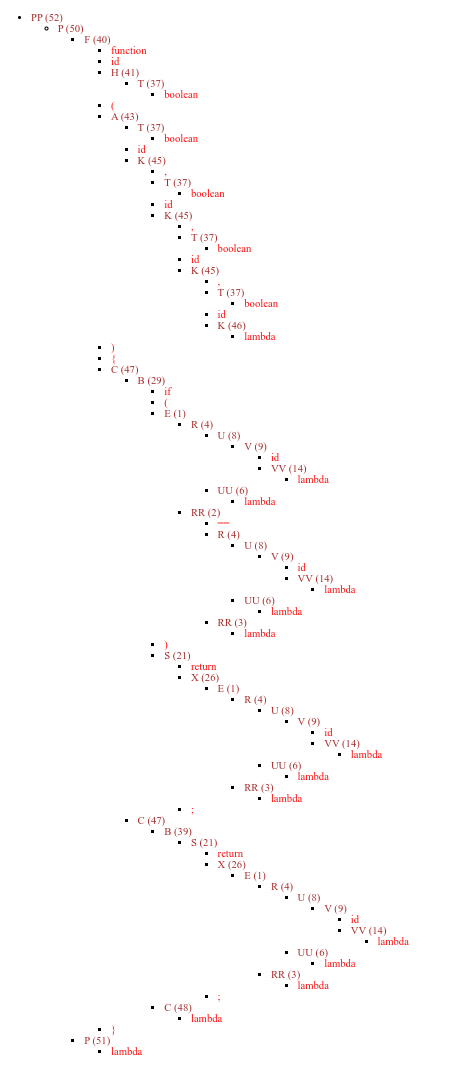
\includegraphics[width=0.6\textwidth]{arbol1.png}

\subsection{Prueba Funcional 2}
Código fuente:
\lstinputlisting[language=JavaScript]{ficheroFuente2.txt}
\hspace{\parindent} Fichero de Tokens:
\lstinputlisting[language=JavaScript]{tokens2.txt}
\hspace{\parindent} Tabla de Símbolos:
\lstinputlisting[language=JavaScript]{ts2.txt}
\hspace{\parindent} Fichero de Parse y Árbol sintáctico:
\lstinputlisting[language=JavaScript]{ficheroParse2.txt}
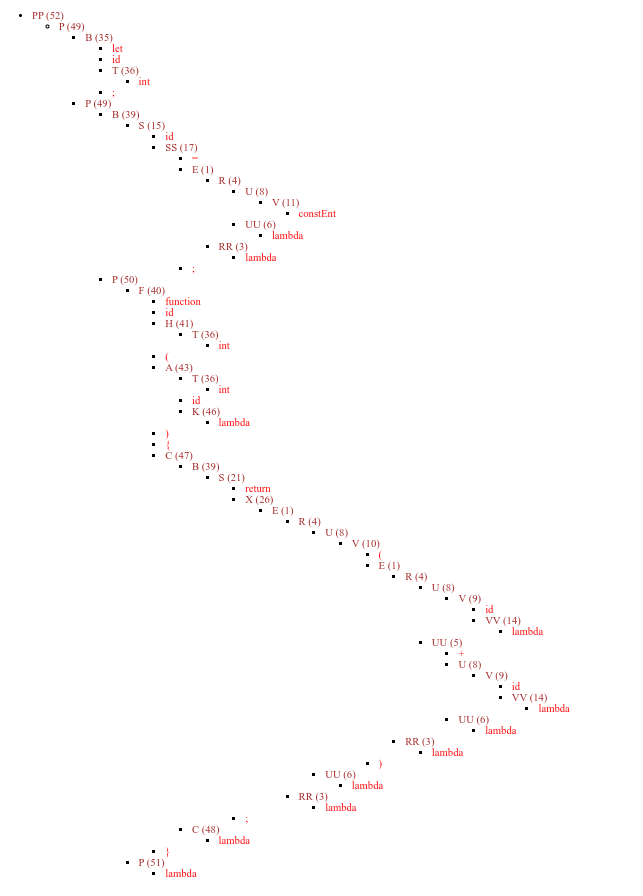
\includegraphics[width=1\textwidth]{arbol2.png}

\subsection{Prueba Funcional 3}
Código fuente:
\lstinputlisting[language=JavaScript]{ficheroFuente3.txt}
\hspace{\parindent} Fichero de Tokens:
\lstinputlisting[language=JavaScript]{tokens3.txt}
\hspace{\parindent} Tabla de Símbolos:
\lstinputlisting[language=JavaScript]{ts3.txt}
\hspace{\parindent} Fichero de Parse y Árbol sintáctico:
\lstinputlisting[language=JavaScript]{ficheroParse3.txt}
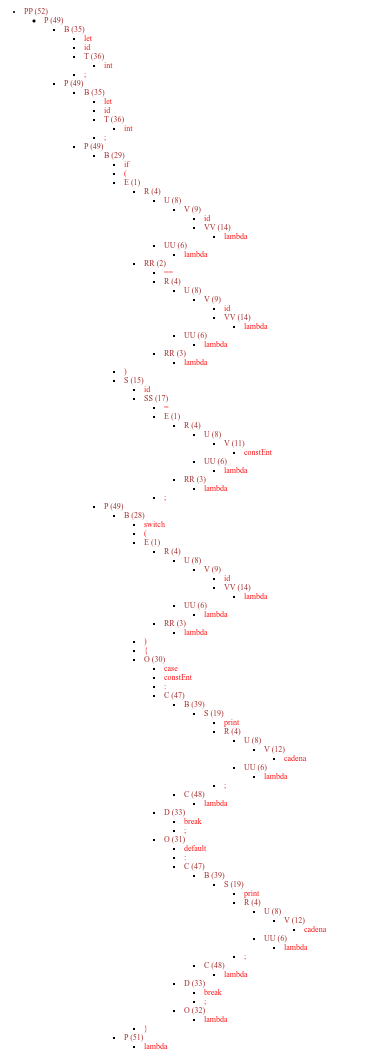
\includegraphics[width=0.5\textwidth]{arbol3.png}

\subsection{Prueba Funcional 4}
Código fuente:
\lstinputlisting[language=JavaScript]{ficheroFuente4.txt}
\hspace{\parindent} Fichero de Tokens:
\lstinputlisting[language=JavaScript]{tokens4.txt}
\hspace{\parindent} Tabla de Símbolos:
\lstinputlisting[language=JavaScript]{ts4.txt}
\hspace{\parindent} Fichero de Parse y Árbol sintáctico:
\lstinputlisting[language=JavaScript]{ficheroParse4.txt}
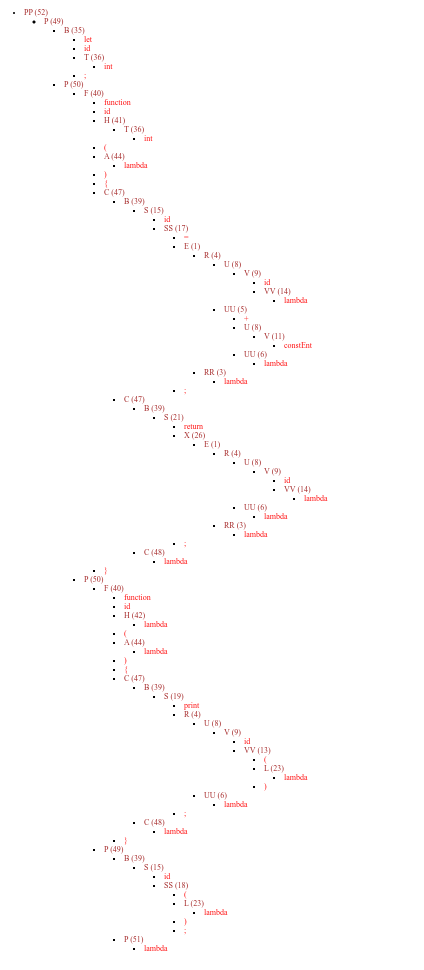
\includegraphics[width=0.65\textwidth]{arbol4.png}

\subsection{Prueba Funcional 5}
Código fuente:
\lstinputlisting[language=JavaScript]{ficheroFuente5.txt}
\hspace{\parindent} Fichero de Tokens:
\lstinputlisting[language=JavaScript]{tokens5.txt}
\hspace{\parindent} Tabla de Símbolos:
\lstinputlisting[language=JavaScript]{ts5.txt}
\hspace{\parindent} Fichero de Parse y Árbol sintáctico:
\lstinputlisting[language=JavaScript]{ficheroParse5.txt}
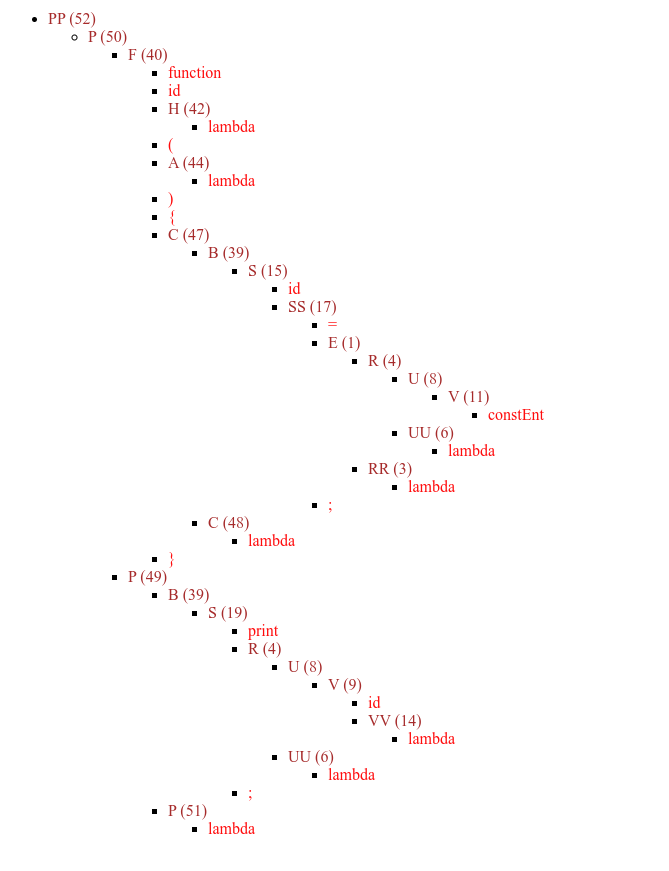
\includegraphics[width=0.85\textwidth]{arbol5.png}

\newpage

\subsection{Prueba No Funcional 1}
Código fuente:
\lstinputlisting[language=JavaScript]{codigoerror1.txt}
Aqui podemos ver dos fallos: el primero es que se intenta realizar una suma sobre valores que no son enteros, en este caso un valor de tipo cadena,
lo cual provoca que el return devuelva un error de tipos incompatibles con la función. Y el siguiente, que se intenta asignar a una variable entera, un valor de tipo cadena.\\
\tab \textcolor{red}{Error en linea: 6 -> Error semantico: el operando + solo admite valores enteros}\\
\tab \textcolor{red}{Error semantico, tipo de funcion no coincide con el valor de return}\\
\tab \textcolor{red}{Error en linea: 8 -> Error semantico: el tipo de variable no coincide con el tipo de valor que se intenta asignar}

\subsection{Prueba No Funcional 2}
Código fuente:
\lstinputlisting[language=JavaScript]{codigoerror2.txt}
En este otro ejemplo, podemos observar que existe un error semantico, al intentar llamar a la función print con un valor booleano, que según la especificación del lenguaje no debería ser posible, además, de tener un error sintáctico por la generación de un case, sin tener un switch previamente.\\
\tab \textcolor{red}{Error en linea: 8 -> Error semantico: Expresion mal formada o variable boolean no admitida}\\
\tab \textcolor{red}{Error Sintáctico: No existe regla para M[P, <palabraReservada, case>].}

\subsection{Prueba No Funcional 3}
Código fuente:
\lstinputlisting[language=JavaScript]{codigoerror3.txt}
En este caso de prueba vemos que al poner una palabra reservada como nombre de una función envía un error, ya que el token que se esperaba era un id, sin embargo, al recibir el token de palabra reservada, no coincide con el de la cima de la pila y acaba la ejecución.\\
\tab \textcolor{red}{Error en linea: 2 -> Error semantico: Expresion incorrecta para la evaluación del switch, debe ser de tipo entero}\\
\tab \textcolor{red}{Error en linea: 3 -> Error semantico: existen uno o multiples cases con la misma constante entera}\\
\tab \textcolor{red}{Error Sintáctico: El terminal de la cima de la pila ``constEnt`` no coincide con el token <cadena, ``hola``> enviado por el AnLex.}

\subsection{Prueba No Funcional 4}
Código fuente:
\lstinputlisting[language=JavaScript]{codigoerror4.txt}
Aqui vemos varios errores semánticos, entre ellos intentar realizar una comparación entre un valor entero y uno de tipo cadena. Otro error por intentar realizar un input sobre una varibale booleana. Y por último un error sintáctico por intentar mandar un token = justo despues de un ;.\\
\tab \textcolor{red}{Error en linea: 3 -> Error semantico: La comparacion solo admite valores enteros}\\
\tab \textcolor{red}{Error en linea: 4 -> Error semantico: La expresion no esta bien formada}\\
\tab \textcolor{red}{Error en linea: 7 -> Error semantico: variable booleana no admitida}\\
\tab \textcolor{red}{Error Sintáctico: No existe regla para M[P, <comparacion, >].}

\subsection{Prueba No Funcional 5}
Código fuente:
\lstinputlisting[language=JavaScript]{codigoerror5.txt}
Aqui encontramos errores léxicos, sintácticos y semánticos. El primero léxico es intentar declarar dos veces una variable con el mismo lexema. El semántico viene dado por intentar evaluar una cadena en un if, cuando este solo admite una expresión booleana. Y el sintáctico viene dado por intentar escribir un número real, lo cual no es admitido por nuestro lenguaje.\\
\tab \textcolor{red}{Error en linea: 2 -> Error léxico: Variable ya declarada}\\
\tab \textcolor{red}{Error en linea: 4 -> Error semantico: La expresion no esta bien formada}\\
\tab \textcolor{red}{Error Sintáctico: No existe regla para M[UU, <constEnt, 2>].}

\end{appendices}

\end{document}